\section{Korrelationsgradanzeige}
Die Korrelationsgradanzeige in Traverso analysiert den linken und rechten Kanal des Masterausgangs, und berechnet deren Korrelationskoeffizienten. Im Gegensatz zu vielen anderen Programmen interpretiert sie den Wert als Ma"s für die Stereobreite des Signals, und stellt den Wert entsprechend dar.

Um zu erklären wozu man die Korrelation überwachen muss nehmen wir an, eine reine Sinuswelle gleicher Frequenz wird sowohl über den rechten als auch über den linken Kanal abgespielt. Werden die beiden Wellen addiert (dies geschieht, wenn das Signal Mono-geschaltet wird, oder wenn sich die Signale in der Luft überlagern), so entsteht ein Summensignal, das je nach Phasenunterschied der beiden Wellen Interferenzerscheinungen aufweist. Das hei"st, wenn zwei positive Werte addiert werden, entsteht ein grö"serer Wert, aber wenn ein positiver und ein negativer Wert summiert werden, entsteht ein Wert mit kleinerem Betrag als die Beträge der Summanden. In einigen Fällen kann dies sogar zu kompletter Auslöschung des Signals führen (\FigB\ \ref{fig_interference}).

\begin{figure}
	\centering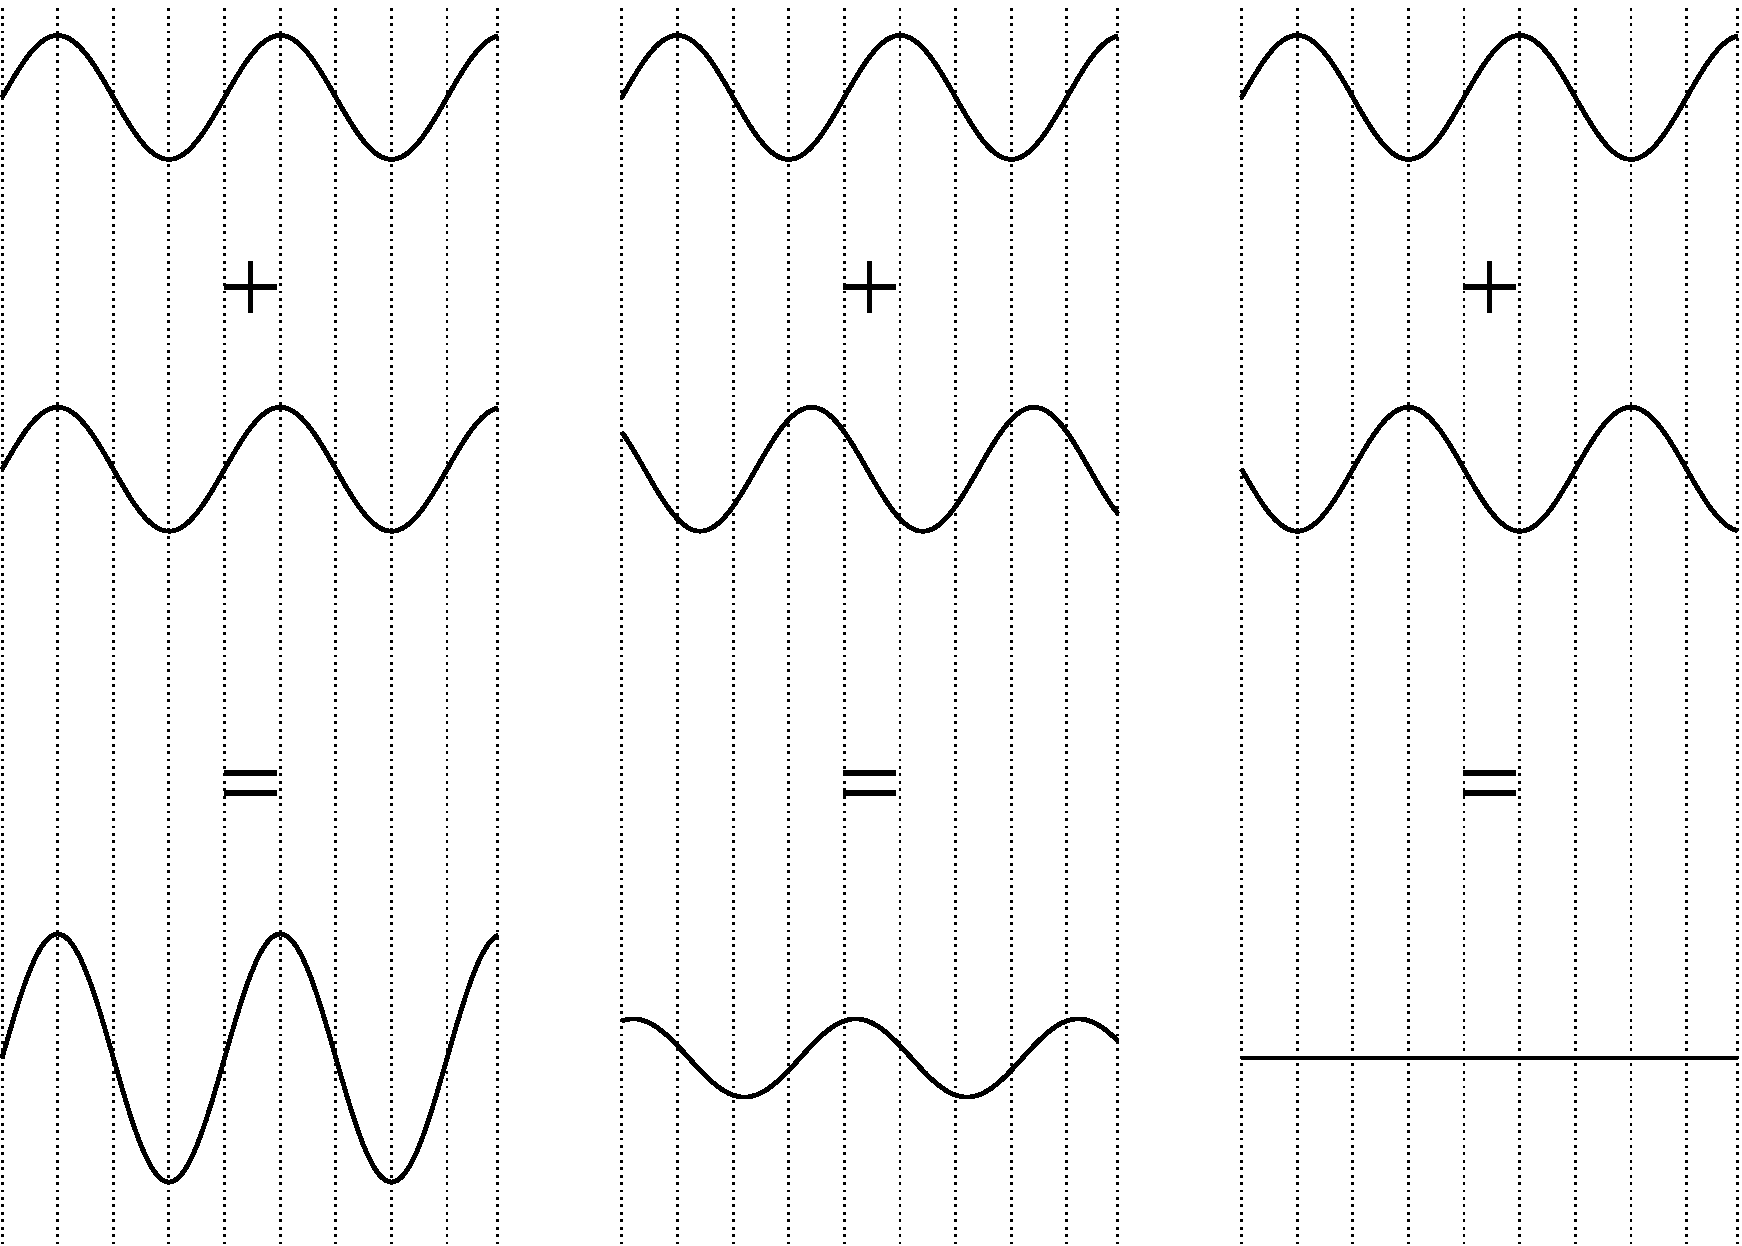
\includegraphics[width=0.8\textwidth]{images/sine01}
	\caption{Werden zwei Sinuswellen addiert, entstehen Interferenzen die entweder zu einer Verstärkung (in Phase, links), einem mehr oder weniger unveränderten Signal (unkorreliert, mitte), oder zu Auslöschung führen können (au"ser Phase, rechts).}
	\label{fig_interference}
\end{figure}

Enthalten die beiden Kanäle komplexere Audiodaten, zum Beispiel Musik oder Sprache, wirken solche Auslöschungen nicht auf das ganze Signal, sondern nur auf gewisse Frequenzbereiche. Der Klang wird dadurch ,,hohl'' oder anderweitig verändert. Solche Effekte sind natürlich in keiner qualitativ hochwertigen Produktion akzeptabel. Normalerweise können sie leicht durch Probehören identifiziert werden, doch bieten heutzutage Analyseprogramme visuelle Darstellungen von Audiosignalen auf vielfältige Weise, was als gro"ser Vorteil gegenüber analogen Lösungen gewertet wird. Es gibt unterschiedliche Arten der Darstellung von Korrelationskoeffizienten. Um zu verstehen, wie die Korrelationsgrad-Darstellung in Traverso zustande kommt und zu interpretieren ist, müssen wir die Berechnung noch etwas genauer betrachten.

Der Grad der Korrelation wird grundsätzlich über den \emph{linearen Korrelationskoeffizienten} $r$ bestimmt, der über eine Reihe von Wertepaaren $(x_i,y_i)$ berechnet wird:
\[
r = \frac{\sum\limits_{i}(x_i - \bar{x})(y_i - \bar{y})}{\sqrt{\sum\limits_{i}(x_i - \bar{x})^2} \sqrt{\sum\limits_{i}(y_i - \bar{y})^2}}
\]
$r$ reicht von $-1.0$ bis $1.0$. Ein Wert von $r = 1.0$ bedeutet, dass das linke und rechte Signal perfekt korrelieren. Das Mastersignal wäre mono in diesem Fall, da es keine Phasendifferenz zwischen dem linken und rechten Signal gibt. Je mehr Unterschiede es gibt, desto tiefer wird der Korrelationskoeffizient. Bei vollkommen unkorrelierten Signalen wird $r = 0.0$. Dies bedeutet, dass es keinerlei Ähnlichkeit zwischen dem linken und rechten Signal gibt. Solch ein Signal produziert ein weites Stereobild, jedoch ohne Gefahr von Phasenauslöschungen. Erst wenn man die Unterschiede der beiden Signale weiter ,,vergrö"sert'', indem ein Kanal zum inversen Signal des anderen wird, besteht eine erhöhte Gefahr von Phasenauslöschungen. $r$ wird in diesem Fall negativ.

Die Korrelationsgradanzeige in Traverso (Menü ,,Ansicht $\rightarrow$ Korrelationsanzeige'') verwendet eine intuitive Darstellung, die anstelle eines numerischen Wertes den Korrelationskoeffizienten in ein Ma"s für die Stereobreite des Signals abbildet (\FigB\ \ref{fig_cmeter01}). Ein Gradient erstreckt sich zwischen zwei Linien, die jeweils den linken und rechten Kanal markieren. Verläuft der Gradient von Linie zu Linie, hat das Signal das breiteste Stereobild, das keine Phasenauslöschungen produziert ($r = 0.0$). Solange sich der Gradient nicht über die beiden Linien heraus erstreckt, tritt keine negative Korrelation auf. Erstreckt er sich jedoch über die Linien hinaus bedeutet dies, dass $r$ negativ ist und Phasenauslöschungen auftreten. Das Stereobild klingt dann unnatürlich weit und hohl. Dies gilt es auf jeden Fall zu vermeiden. Ein Mono-Signal dagegen führt dazu, dass sich der Gradient auf eine Linie verengt.

\begin{figure}
	\centering
	\subfigure[Stereo, $r = 0.0$]{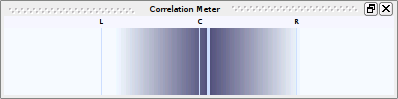
\includegraphics[width=0.7\textwidth]{images/cmeter1}}
	\subfigure[Mono, $r = 1.0$]{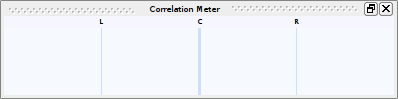
\includegraphics[width=0.7\textwidth]{images/cmeter2}}
	\subfigure[Phasenauslöschung, $r = -1.0$]{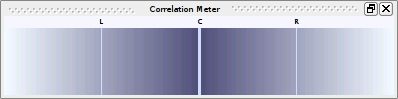
\includegraphics[width=0.7\textwidth]{images/cmeter4}}
	\caption{Die Korrelationsgradanzeige in Traverso zeigt den Korrelationskoeffizienten des Masterausgangs als Gradient zwischen zwei vertikalen Linien, die jeweils den linken und rechten Kanal darstellen. Verläuft der Gradient genau von L bis R, ist das Signal völlig unkorreliert ($r = 0.0$), und es besitzt ein sehr breites Stereobild (oben). Reduziert sich der Gradient auf eine Linie, sind die Daten perfekt korreliert ($r = 1.0$), was bedeutet, dass das Ausgangssignal mono erscheint (mitte). Erstreckt sich der Gradient über die L und R Linien hinaus, wird die Korrelation negativ und das Risiko von Phasenauslöschungen im Monosignal steigt an (unten).}
	\label{fig_cmeter01}
\end{figure}

Die Korrelationsgradanzeige kann auch dazu verwendet werden, die Balance des Signals zu justieren. Für ein zentriertes Signal, das auf beiden Kanälen etwa gleich laut klingt, sollte die Zenterlinie des Gradientes um die Mittenlinie herumtanzen.

Da sich der Gradient normalerweise zwischen den beiden Linien L und R befindet, kann man mittels \sact{M} den horizontalen Anzeigebereich verändern. Mehrmaliges drücken von \sact{M} setzt den Wert wieder auf den kompletten Bereich zurück.

\section{FFT-Spektrumsanzeige}
Eine auf der Fast Fourier Transformation (FFT) basierende Spektrumsanzeige gehört heutzutage zur Standardausrüstung einer digitalen Audioworkstation. Die FFT-Spektrumsanzeige in Traverso wird über das Menü ,,Ansicht $\rightarrow$ FFT-Frequenzspektrum'' aufgerufen. Sie wurde als Dock-Fenster realisiert, das man entweder in das Hauptfenster integrieren oder frei auf dem Bildschirm platzieren kann.

Die FFT-Spektrumsanzeige analysiert den Master-Ausgang und zerlegt das Audiosignal in Frequenzbänder. Jedes Band zeigt den höchsten Betrag $dB_{links} + dB_{rechts}$ innerhalb seines Bereichs (\FigB\ \ref{fig_fft1}). Ein Einstellungsdialog kann über den Befehl \sact{E} geöffnet werden, oder über das Kontextmenü \sact{Q}.

\begin{figure}
	\centering
	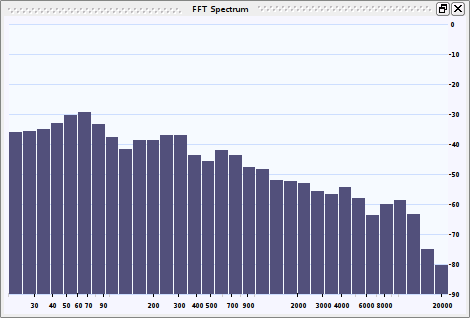
\includegraphics[width=0.6\textwidth]{images/fft1}
	\caption{Die FFT-Spektrumsanzeige zerlegt das Mastersignal in seine Frequenzen.}
	\label{fig_fft1}
\end{figure}

Der Konfigurationsdialog (\FigB\ \ref{fig_fft3}) ermöglicht es, den angezeigten Wertebereich in dB und Frequenzen zu definieren. Das für Menschen hörbare Spektrum reicht ungefähr von 20 bis 18000~Hz. CDs speichern einen Bereich von 20 bis 22050~Hz. Der angezeigte Frequensbereich sollte also in den meisten Fällen etwa diese Frequenzen abdecken. Für die Lautstärke gelten in der Regel eine Obergrenze von $-6$ bis $+6$~dB und eine Untergrenze im Bereich von $-60$ bis $-120$~dB. Die Anzahl Frequenzbänder kann frei gewählt werden, man sollte jedoch beachten, dass die Prozessorauslastung mit der Anzahl Bänder zunimmt, und ab $\geq 128$ erheblich werden kann.

Die Funktion ,,Durchschnittskurve anzeigen'' oder \sact{M} aktiviert eine Kurve, die während des Abspielens die gemessenen Frequenzen summiert und den Durchschnitt berechnet. Wird der Transport gestoppt und wieder gestartet, beginnt die Berechnung von neuem. Die Kurve kann auch durch drücken von \sact{L} zurückgesetzt werden. Sobald Durschnittswerte vorhanden sind, können diese auch exportiert werden. Als Exportformate stehen eine ASCII-Tabelle oder \texttt{grace} zur Verfügung. Letzteres kann mit dem Programm XmGrace geöffnet werden.

FFT-relevante Parameter können im Abschnitt ,,Erweitert'' im Einstellungsdialog geändert werden. Die Grö"se der FFT bestimmt die tiefste Frequenz, die von der Analyse noch erfasst wird. Je grö"ser die FFT, desto tiefer die Frequenz, aber desto höher wird die Speicher- und Prozessorbelastung. Die tiefste Frequenz wird wie folgt berechnet:
\[
f_{min} = \frac{\textrm{Samplerate}}{\textrm{FFT size}}
\]
Die \emph{tiefste} Frequenz bei einer FFT-Grö"se von 1024 Samples beträgt demnach bei einer Samplerate von 44100~Hz genau 43.1~Hz. Vergrö"sert man die FFT auf 2048 Samples, liegt die tiefste Frequenz bei 21.5~Hz. Die \emph{höchste} gemessene Frequenz berechnet man durch
\[
f_{max} = 0.5 \cdot \textrm{Samplerate}
\]
Für Audiodaten mit einer Samplerate von 44100~Hz liegt sie daher fest bei 22050~Hz.

Die Fensterungsfunktion kann in diesem Dokument nicht mit einfachen Worten erklärt werden, und es empfiehlt sich in den meisten Fällen, die ,,Hanning''-Funktion zu verwenden.

\begin{figure}
	\centering
	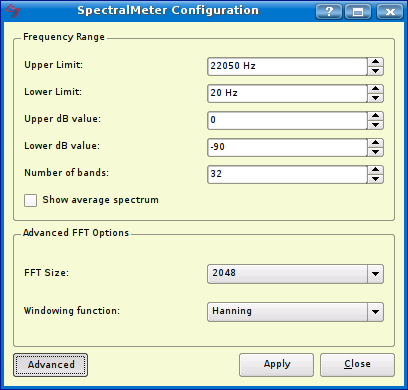
\includegraphics[width=0.7\textwidth]{images/fft3}
	\caption{Über einen Konfigurationsdialog (\sact{E}) kann man diverse Parameter einstellen.}
	\label{fig_fft3}
\end{figure}

\emph{Wichtig:} Für sehr grosse FFTs wird die Darstellung des Frequenzspektrums sehr ruckelig. Dies ist nicht unbedingt durch die erhöhte Prozessorbelastung bedingt, sondern durch die Tatsache, dass die FFT-Puffer einige Zeit brauchen, bis sie mit neuen Audiodaten gefüllt sind. In dieser Zeit wird das Spektrum nicht neu gezeichnet.

\section{Externe Bearbeitung}
Traverso bietet die Möglichkeit, Audioclips extern durch Zusatzprogramme wie ,,sox'' \cite{sox} zu bearbeiten. Dies ermöglicht die Verwendung von zusätzlichen Effekten, was besonders für Samplerate-Konversionen, Entfernung von Gleichspannung, Phaseninvertierung etc. geeignet ist. Auf Linux-Plattformen muss das Programm ,,sox'' installiert werden, das jedoch in allen gängigen Distributionen über das offizielle Repositorium verfügbar ist. Auf Windows und OS X wird das Programm mit Traverso automatisch installiert.

\begin{figure}
	\centering
	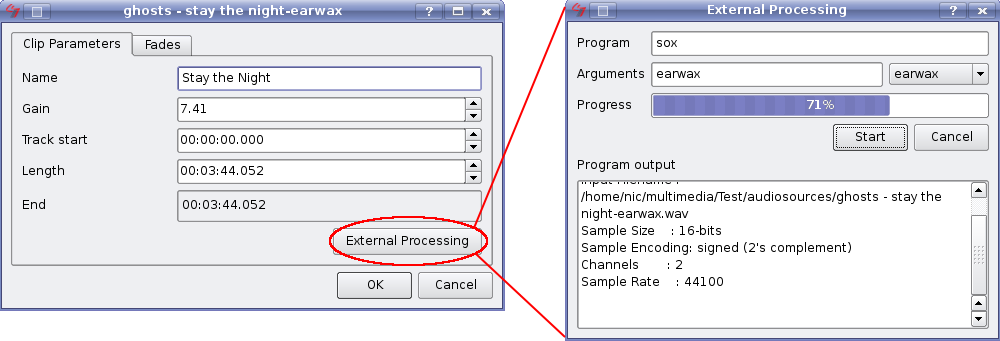
\includegraphics[width=\textwidth]{images/external00}
	\caption{Drückt man auf einem Audioclip \sact{E}, so öffnet sich ein Dialog (links). Drückt man darin den Knopf ,,Externe Bearbeitung'', öffnet sich ein weiterer Dialog (rechts), in dem man zahlreiche Effekte auf die Audiodatei anwenden kann.}
	\label{fig_external01}
\end{figure}

Ein Editor kann durch drücken von \sact{E} auf einem Audioclip geöffnet werden (\FigB~\ref{fig_external01}). Drückt man darin den Knopf ,,Externe Bearbeitung'', öffnet sich ein weiterer Dialog, in dem die Einstellungen dazu vorgenommen werden (\FigB~\ref{fig_external01} right). Lasst das ,,Programm'' jeweils auf ,,sox'' eingestellt, und wählt einen Effekt aus der ,,Argumente''-Box aus. Lasst den Namen des Argumentes in der Zeile stehen und hängt eure eigenen Argumente an. Verwirrt? Gut, dann betrachten wir ein Beispiel. Nehmen wir an wir wollen die Phase der Datei meinedatei.wav invertieren. Importiert sie dazu in Traverso und drückt \sact{E} auf dem Clip, danach den Knopf ,,Externe Bearbeitung'' im Bearbeitungsdialog. Lasst ,,sox'' als Programm eingestellt und wählt als Effekt ,,vol'' aus. Das erste Argument wird auf ,,vol'' gesetzt. Gemä"s der sox-Dokumentation invertiert man die Phase, indem man ,,vol'' auf $-1.0$ stellt. Schreibt also hinter das automatisch eingesetzte ,,vol'' noch ,,$-1.0$'' (ohne Anführungszeichen). Dann drückt ,,Start'' und wartet, bis der Prozess vorbei ist. Der Clip in Traverso wird automatisch durch die neue Wave-Datei ersetzt, die den Namen ,,meinedatei-vol -1.0.wav'' trägt. Die neue Datei wird im Verzeichnis ,,audiosources'' in eurem Projektverzeichnis gespeichert, unabhängig davon wo die ursprüngliche Datei lag. Durch die Umbenennung wird die Originaldatei nie überschrieben. Weitere Informationen zu sox-Effekten findet man in der man-page, die auf Linux durch Eingabe von ,,man:sox'' in Konqueror, oder ,,man sox'' in einem Terminal geöffnet wird.